\documentclass{standalone}

\usepackage{pgfplots}
\pgfplotsset{compat=newest}

\begin{document}
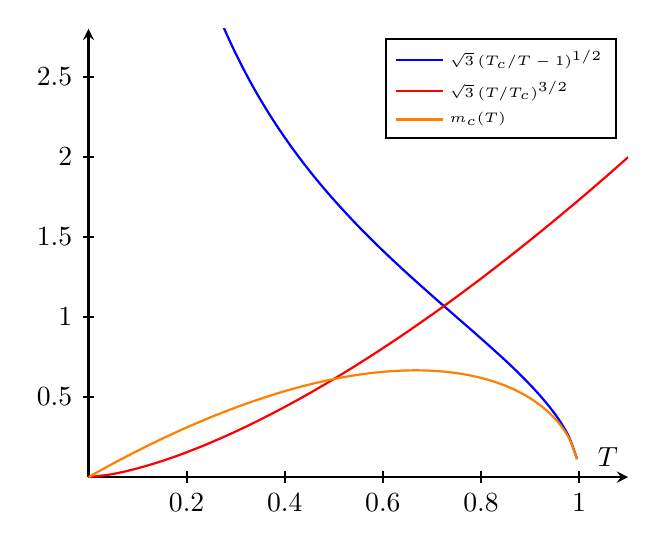
\begin{tikzpicture}
  \begin{axis}[
      xlabel = $T$,
      smooth,thick,
      domain=0:1.1,
      ymax=2.8,
      axis lines = center,
      every tick/.style = {thick},
      legend cell align=left,
      legend style={font=\tiny}]

    \def\Tc{1}
    \addplot[color=blue,samples=75]{sqrt(3)*(\Tc/x - 1)^(1/2)};
    \addplot[color=red]{sqrt(3)*(x/\Tc)^(3/2)};
    \addplot[color=orange,samples=75]{sqrt(3)*(x/\Tc)^(3/2)*(\Tc/x - 1)^(1/2)};

    \legend{$\sqrt{3} \left(T_c/T - 1\right)^{1/2}$,
      $\sqrt{3} \left(T/T_c\right)^{3/2}$,
      $m_c(T)$}

  \end{axis}
\end{tikzpicture}
\end{document}